\documentclass[12pt]{article}

\usepackage{graphicx}
\usepackage{paralist}
\usepackage{amsfonts}
\usepackage{amsmath}
\usepackage{hhline}
\usepackage{booktabs}
\usepackage{multirow}
\usepackage{multicol}
\usepackage{url}

\oddsidemargin -10mm
\evensidemargin -50mm
\textwidth 180mm
\textheight 200mm
\renewcommand\baselinestretch{1.0}
\newcommand{\specialcell}[2][l]{%
  \begin{tabular}[#1]{@{}l@{}}#2\end{tabular}}
\pagestyle {plain}
\pagenumbering{arabic}

\newcounter{stepnum}

%% Comments

\usepackage{color}

\title{\huge{Safety Net} \\ \vspace{3mm} \large{Version 1.4} \\ \vspace{3mm} McMaster University \\ COMPSCI 2XB3 L03}
\author{Group 2: Suleyman Kiani, Sunny Bhatt, Nikola Milanovic, Senan Gohar} \date{}

\begin{document}

\maketitle
\vspace{5mm}
\section*{Summary}
NYC Safety Net for Tourists and Visitors is a desktop application that maps crime data to
different regions of New York City, using NYPD arrest data of approximately four million crimes. Users can filter
for specific crimes in designated areas of NYC to learn about safety with respect to certain crimes. The
application assists tourists travelling to NYC by informing them safe areas to stay, ultimately helping them
save money by staying in safe areas outside of Manhattan. It also provides valuable information to Real Estate
Investors, as they can analyze crime data in areas and evaluate likelihood of investments to flourish due
to gentrification, etc. Features of the application include comparing crime frequency and types of crime
between the bureaus of NYC, comparing crime during different time periods, getting crime data at
a specific address, and finding the safest path between two areas of the city.

\newpage

\section* {Revisions}
\subsection*{Revision history}
\subsubsection*{1.1}
Switched to using OpenCSV to parse the crime dataset, improving performance.
\subsubsection*{1.2}
User interface improvements, now displaying frequency of crimes and limiting results to top 5 or 10 with an option to display all results.
\subsubsection*{1.3}
Introduction of the location lookup feature, utilizing a geocoding API from LocationIQ.
\subsubsection*{1.4}
Introduction of the safest path feature, implementing Dijkstra's shortest path algorithm.

\vspace{10mm}
\subsection*{Consent}
By virtue of submitting this document we electronically sign and date that the work being submitted by all the
individuals in the group is their exclusive work as a group and we consent to make available the application
developed through CS2XB3 project, the reports, presentations, and assignments (not including my
name and student number) for future teaching purposes.
\vspace{5mm}
\\
\newpage

\section* {Contributions}

\begin{tabular}{| l | l | l |}
    \hline
    \textbf{Name} & \textbf{Role(s)} & \textbf{Contributions}\\
    \hline
    Sunny Bhatt & \specialcell{Developer\\Tester} & CSV parsing, location crime lookup, unit tests, Map MIS \\
    \hline
    Nikola Milanovic & \specialcell{Team leader\\Developer\\Maintainer} & ADT's, Map, Interface, ShortestPath, UML, Design\\
    \hline
    Suleyman Kiani & Developer & Module design, Application Design, MIS\\
    \hline
    Senan Gohar & Developer & \specialcell{User interface, Java documentation, architecture design}\\
    \hline
    \end{tabular}

\newpage

\section* {Application level UML diagram}

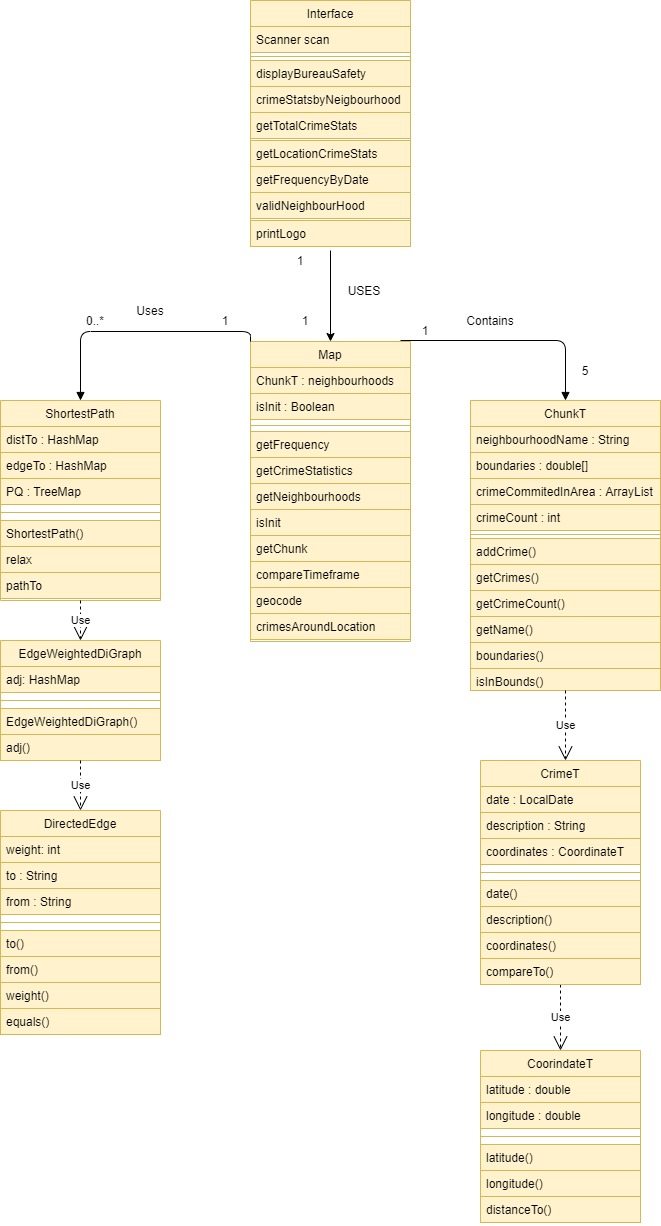
\includegraphics[scale = 0.5]{UML.jpg}

\section* {Coordinate ADT Module}

\subsection*{Module}

CoordinateT

\subsection* {Uses}

N/A

\subsection* {Syntax}

\subsubsection* {Exported Constants}

None

\subsubsection* {Exported Types}

CoordinateT = ? \\


\subsubsection* {Exported Access Programs}

\begin{tabular}{| l | l | l | l |}
\hline
\textbf{Routine name} & \textbf{In} & \textbf{Out} & \textbf{Exceptions}\\
\hline
CoordinateT & $\mathbb{R}$, $\mathbb{R}$ & CoordinateT & \\
\hline
latitude & ~ & $\mathbb{R}$ & ~\\
\hline
longitude & ~ & $\mathbb{R}$ & ~\\
\hline
distanceTo & CoordinateT & $\mathbb{R}$ & ~\\
\hline
\end{tabular}

\subsection* {Semantics}

\subsubsection* {State Variables}

$lat$: $\mathbb{R}$\\
$lon$: $\mathbb{R}$


\subsubsection* {Considerations}

The constructor CoordinateT is called for each object instance before any other
access routine is called for that object.  The constructor cannot be called on
an existing object.

\subsubsection* {Access Routine Semantics}

CoordinateT($lat, lon$):
\begin{itemize}
\item transition: $lat, lon := latitude, longitude$
\item output: $out := \mathit{self}$
\item exception: None
\end{itemize}

\noindent latitude():
\begin{itemize}
\item output: $out := lat$
\item exception: None
\end{itemize}

\noindent longitude():
\begin{itemize}
\item output: $out := lon$
\item exception: None
\end{itemize}

\noindent distanceTo(c):
\begin{itemize}
\item output: $\textnormal{\small{Great-circle distance from self to c using the haversine formula}}$
\item exception: None
\end{itemize}


\newpage


\section* {Crime ADT Module}

\subsection*{Template Module}

CrimeT

\subsection* {Uses}

CoordinateT

\subsection* {Syntax}

\subsubsection* {Exported Types}

CrimeT = ?

\subsubsection* {Exported Access Programs}

\begin{tabular}{| l | l | l | l |}
\hline
\textbf{Routine name} & \textbf{In} & \textbf{Out} & \textbf{Exceptions}\\
\hline
CrimeT & LocalDate, String, CoordinateT & CrimeT & \\
\hline
date & ~ & LocalDate & ~\\
\hline
description & ~ & String & ~\\
\hline
coordinate & ~ & CoordinateT & ~\\
\hline
compareTo & CrimeT & $\mathbb{Z}$ & ~\\
\hline
\end{tabular}

\subsection* {Semantics}

\subsubsection* {State Variables}

$date$: LocalDate\\
$description$: String\\
$coordinates$: CoordinateT


\subsubsection* {Access Routine Semantics}

CrimeT($d, desc, c$):
\begin{itemize}
\item transition: $date, description, coordinates := d, desc, c$
\item output: $out := \mathit{self}$
\item exception: None
\end{itemize}

\noindent date():
\begin{itemize}
\item output: $out := date$
\item exception: None
\end{itemize}

\noindent description():
\begin{itemize}
\item output: $out := description$
\item exception: None
\end{itemize}

\noindent coordinate():
\begin{itemize}
\item output: $out := coordinates$
\item exception: None
\end{itemize}

\noindent compareTo(that):
\begin{itemize}
\item output: $out := \textnormal{date().compareTo(that.date())}$
\item exception: None
\end{itemize}

\newpage

\section* {Chunk ADT Module}

\subsection* {Generic Template Module}

ChunkT

\subsection* {Uses}

CrimeT

\subsection* {Syntax}

\subsubsection* {Exported Types}

ChunkT = ?

\subsubsection* {Exported Constants}

None

\subsubsection* {Exported Access Programs}

\begin{tabular}{| l | l | l | p{6cm} |}
\hline
\textbf{Routine name} & \textbf{In} & \textbf{Out} & \textbf{Exceptions}\\
\hline
ChunkT & name, $\mathbb{R}$, $\mathbb{R}$, $\mathbb{R}, \mathbb{R}$ & ChunkT & ~\\
\hline
addCrime & CrimeT & ~ & ~\\
\hline
getCrimes & ~ & seq of CrimeT & ~\\
\hline
getCrimeCount & ~ & $\mathbb{Z}$ & ~\\
\hline
getName & ~ & String & ~\\
\hline
boundaries & ~ & seq of $\mathbb{R}$ & ~\\
\hline
isInBounds & CrimeT & $\mathbb{B}$ & ~\\
\hline
\end{tabular}

\subsection* {Semantics}

\subsubsection* {State Variables}

neighbourhoodName: String\\
boundaries: seq of $\mathbb{R}$\\
crimesCommitedInArea: seq of CrimeT\\
crimeCount: $\mathbb{Z}$


\subsubsection* {Access Routine Semantics}

ChunkT($name, left, right, up, down$):
\begin{itemize}
\item transition: $neighbourhoodName := name$\\
$boundaries[0], boundaries[1], boundaries[2], boundaries[3] = left, right, up, down$
\item output: $\mathit{out} := \mathit{self}$
\item exception: None
\end{itemize}

\noindent addCrime($crime$):
\begin{itemize}
\item transition: $crimesCommitedInArea.add(crime)$\\$crimeCount++$
\item exception: None
\end{itemize}

\noindent getCrimes():
\begin{itemize}
\item transition: None
\item output: $out := crimesCommitedInArea$
\item exception: None
\end{itemize}

\noindent getCrimeCount():
\begin{itemize}
\item transition:
\item output: $out := crimeCount$
\item exception: None
\end{itemize}

\noindent getName():
\begin{itemize}
\item transition: None
\item output: $out := neighbourHoodName$
\item exception: None
\end{itemize}

\noindent boundaries():
\begin{itemize}
\item transition:
\item output: $out := boundaries$
\item exception: None
\end{itemize}

\noindent isInBounds(crime):
\begin{itemize}
\item transition: None
\item output: $\textnormal{\small{Returns true if crime.coordinates() is located within the four bounds of this chunk}}$
\item exception: None
\end{itemize}

\newpage

\section* {Map Abstract Object Module}

\subsection*{Abstract Object}

Map

\subsection* {Uses}

ChunkT, CrimeT, CoordinateT

\subsection* {Syntax}

\subsubsection* {Exported Types}

None

\subsubsection* {Exported Access Programs}

\begin{tabular}{| l | l | l | l |}
\hline
\textbf{Routine name} & \textbf{In} & \textbf{Out} & \textbf{Exceptions}\\
\hline
init & ~ & ~ & \\
\hline
getFrequency & $\mathbb{B}$ & seq of String & ~\\
\hline
getCrimeStatistics & $\mathbb{B}$ & map of String to Integer & ~\\
\hline
getCrimeStatistics & $\mathbb{B}$, String & map of String to Integer & ~\\
\hline
getCrimeStatistics & $\mathbb{B}$, seq of CrimeT & map of String to Integer & ~\\
\hline
getNeighbourhoods & ~ & seq of ChunkT & ~\\
\hline
isInit & ~ & $\mathbb{B}$ & ~\\
\hline
getChunk & String & ChunkT & ~\\
\hline
compareTimeframe & LocalDate, LocalDate & seq of CrimeT & ~\\
\hline
assignCrimeToChunk & CrimeT & ~ & ~\\
\hline
geocode & String & CoordinateT & ~\\
\hline
crimesAroundLocation & CoordinateT, $\mathbb{R}$ & seq of CrimeT & ~\\
\hline
\end{tabular}

\subsection* {Semantics}

\subsubsection* {State Variables}

$isInit$: $\mathbb{B}$\\
$neighbourhoods$: seq of ChunkT\\

\subsubsection* {Access Routine Semantics}

init():
\begin{itemize}
\item transition: \textnormal{\small{Initializes NYC's five bureaus to chunks and parses a CSV file of crimes into those chunks. }}
\item exception: None
\end{itemize}

\noindent getFrequency(descending):
\begin{itemize}
\item output: \textnormal{\small{Returns a sequence of neighbourhood names sorted by the number of crimes in the corresponding chunks. If descending is true, the sequence is sorted in descending order, else ascending order. }}
\item exception: None
\end{itemize}

\noindent getCrimeStatistics(descending : $\mathbb{B}$):
\begin{itemize}
\item output: \textnormal{\small{Returns a map of crime description mapped to frequency of the crime across all neighbourhoods. If \textit{descending} is true, the sequence is sorted in descending order of frequency, else ascending order. }}
\item exception: None
\end{itemize}

\noindent getCrimeStatistics(descending : $\mathbb{B}$, neighbourHoodName : String):
\begin{itemize}
\item output: \textnormal{\small{Returns a map of crime description mapped to frequency of the crime in the neighbourhood \textit{neighbourhoodName}. If \textit{descending} is true, the sequence is sorted in descending order of frequency, else ascending order. }}
\item exception: None
\end{itemize}

\noindent getCrimeStatistics(descending : $\mathbb{B}$, crimes : seq of CrimeT):
\begin{itemize}
\item output: \textnormal{\small{Returns a map of crime description mapped to frequency of the crime in a given sequence of crimes. If \textit{descending} is true, the sequence is sorted in descending order of frequency, else ascending order. }}
\item exception: None
\end{itemize}

\noindent getNeighbourhoods():
\begin{itemize}
\item output: out := neighbourhoods
\item exception: None
\end{itemize}

\noindent isInit():
\begin{itemize}
\item output: out := isInit
\item exception: None
\end{itemize}

\noindent getChunk(neighbourHoodName):
\begin{itemize}
\item output: \textnormal{\small{Returns the chunk with name \textit{neighbourHoodName}.}}
\item exception: None
\end{itemize}

\noindent compareTimeframe(start, end):
\begin{itemize}
\item output: \textnormal{\small{Returns a sequence of crimes that occured between the dates \textit{start} and \textit{end}.}}
\item exception: None
\end{itemize}

\noindent assignCrimeToChunk(crime):
\begin{itemize}
\item transition: \textnormal{\small{Adds \textit{crime} to the chunk its coordinates lie within.}}
\item exception: None
\end{itemize}

\noindent geocode(address):
\begin{itemize}
\item transition: \textnormal{\small{Returns a GPS coordinate given \textit{address}, a string description of the location.}}
\item exception: None
\end{itemize}

\noindent crimesAroundLocation(location, radius):
\begin{itemize}
\item transition: \textnormal{\small{Returns a sequence of crimes with coordinates within \textit{radius} kilometers of \textit{location}}}
\item exception: None
\end{itemize}


\newpage

\section* {ShortestPath ADT Module}

\subsection*{Template Module}

ShortestPath

\subsection* {Uses}

EdgeWeightedDiGraph

\subsection* {Syntax}

\subsubsection* {Exported Types}

ShortestPath = ?

\subsubsection* {Exported Access Programs}

\begin{tabular}{| l | l | l | l |}
\hline
\textbf{Routine name} & \textbf{In} & \textbf{Out} & \textbf{Exceptions}\\
\hline
ShortestPath() & EdgeWeightedDiGraph, String & ~ & ~\\
\hline
relax & EdgeWeightedDiGraph, String & ~ & ~\\
\hline
pathTo & String & Stack & ~\\
\hline
\end{tabular}

\subsection* {Semantics}

\subsubsection* {State Variables}

$distTo$: map of String to $\mathbb{R}$\\
$edgeTo$: map of String to DirectedEdge\\
$PQ$: map of $\mathbb{R}$ to String

\subsubsection* {Access Routine Semantics}

ShortestPath(EdgeWeightedDiGraph G, String source):
\begin{itemize}
\item transition: Initializes all the state variables, sets all the distances to
positive infinity except the source and starts Djkstra's algorithm to find the shortest path.
\item output: out := none
\item exception: None
\end{itemize}

\noindent relax(EdgeWeightedDiGraph G, String vertex):
\begin{itemize}
\item transition: Edge relaxation for the given vertex.
\item output: out := none
\item exception: None
\end{itemize}

\noindent pathto(String v):
\begin{itemize}
\item output: out := A stack of directed edges that represents the path from the source
vertex to the provided vertex v if such a path exists.
\item exception: None
\end{itemize}

\newpage

\section* {EdgeWeightedDiGraph ADT Module}

\subsection*{Template Module}

EdgeWeightedDiGraph

\subsection* {Uses}

DirectedEdge

\subsection* {Syntax}

\subsubsection* {Exported Types}

EdgeWeightedDiGraph = ?

\subsubsection* {Exported Access Programs}

\begin{tabular}{| l | l | l | l |}
\hline
\textbf{Routine name} & \textbf{In} & \textbf{Out} & \textbf{Exceptions}\\
\hline
EdgeWeightedDiGraph() & ~ & ~ & ~\\
\hline
adj & ~ & map of String to (seq of DirectedEdge) & ~\\
\hline
\end{tabular}

\subsection* {Semantics}

\subsubsection* {State Variables}

adj : map of String to (seq of DirectedEdge)

\subsubsection* {Access Routine Semantics}

EdgeWeightedDiGraph():
\begin{itemize}
\item transition: Creates all the edges for our graph with all the neighbourhoods.
\item output: out := none
\item exception: None
\end{itemize}

adj():
\begin{itemize}
\item output: out := adj
\item exception: None
\end{itemize}

\newpage

\section* {DirectedEdge ADT Module}

\subsection*{Template Module}

DirectedEdge

\subsection* {Uses}

None

\subsection* {Syntax}

\subsubsection* {Exported Types}

DirectedEdge = ?

\subsubsection* {Exported Access Programs}

\begin{tabular}{| l | l | l | l |}
\hline
\textbf{Routine name} & \textbf{In} & \textbf{Out} & \textbf{Exceptions}\\
\hline
DirectedEdge() & String, String, $\mathbb{Z}$ & ~ & ~\\
\hline
to & ~ & String & ~\\
\hline
from & ~ & String & ~\\
\hline
weight & ~ & $\mathbb{Z}$ & ~\\
\hline
equals & DirectedEdge & $\mathbb{B}$ & ~\\
\hline
\end{tabular}

\subsection* {Semantics}

\subsubsection* {State Variables}

to : String\\
from : String\\
weight : $\mathbb{Z}$

\subsubsection* {Access Routine Semantics}

DirectedEdge(to, from ,weight):
\begin{itemize}
\item transition: to, from, weight := to, from , weight
\item output: out := none
\item exception: None
\end{itemize}

to():
\begin{itemize}
\item output: out := to
\item exception: None
\end{itemize}

from():
\begin{itemize}
\item output: out := from
\item exception: None
\end{itemize}

weight():
\begin{itemize}
\item output: out := weight
\item exception: None
\end{itemize}

equals(DirectedEdge other):
\begin{itemize}
\item output: out := $to = other.to() \land from = other.from$
\item exception: None
\end{itemize}

\newpage

\section* {UML state diagram for Interface}

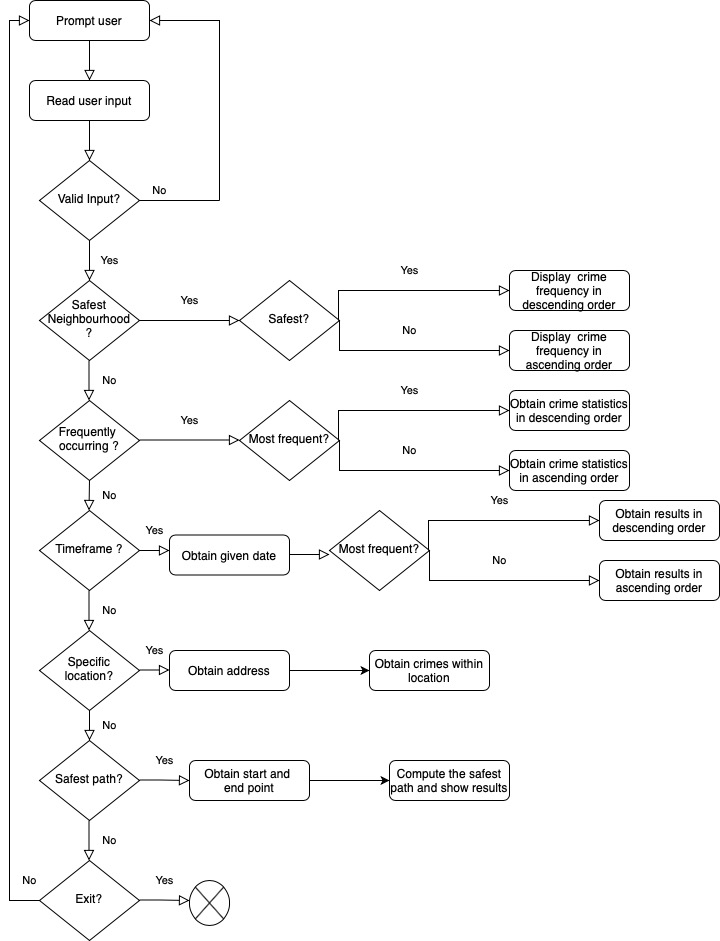
\includegraphics[scale = 0.60]{InterfaceUML.jpg}

\section* {Module descriptions}

\subsection*{Interface}
The interface module is equivalent to the view and controller module in the model-view-controller design. The program user uses this class as an interface to interact with Map and Shortest Path in order to perform a variety of queries.

\subsection*{Map}
This module functions as the model where all the logical processes occur. It provides methods for all the possible queries that a user can search for using the interface module to interact with it. A high-level abstraction of the methods available are:
\begin{itemize}
    \item Obtain the safest/least safe neighbourhoods according to the number of crimes committed within that neighbourhood.
    \item Obtain the most/least occurring crimes within NYC, within a specific neighbourhood or within a given time period.
    \item Obtain the crimes committed within a certain radius of a specified address.
    \item Obtain the safest path from one neighbourhood to another.
\end{itemize}

\subsection*{ShortestPath}
Given a starting point and a destination, obtain the safest path from the two points according to the number of crimes committed in each neighbourhood.

\subsection*{EdgeWeightedDiGraph}
An edge-weighted directed graph with all the neighbourhood connections. The vertices are neighbourhoods and the edges are paths from one neighbourhood to another with the edge-weight being the number of crimes committed within the next vertex.

\subsection*{DirectedEdge}
Standard class representing a directed edge. The vertices are Strings and the weight is an Integer.

\subsection*{ChunkT}
ChunkT represents a neighbourhood and all the information contained within. Chunks are specified by their four boundaries and their name. Chunks also contain information about all the crime statistics contained within their boundaries.

\subsection*{CrimeT}
Represents a crime and contains information about the date of occurrence, crime description, and location. Two crimes are compared according to their date of occurrence.

\subsection*{CoordinateT}
A module for representing coordinates according to latitude and longitude.

\end {document}
